
\section{MOEA/D}\label{sec:background} 


MOEA/D represents a class of population-based meta-heuristics for solving Multi Objective Problems (MOPs).

It is based on decomposition - one kind of scalarizing function
One multi-objective problem becomes various single-objective sub-problems.
All sub-problems are solved in parallel.
A decomposition strategy generates weight vectors that defines the sub-problems.

\begin{figure*}[!t]
	\centering
	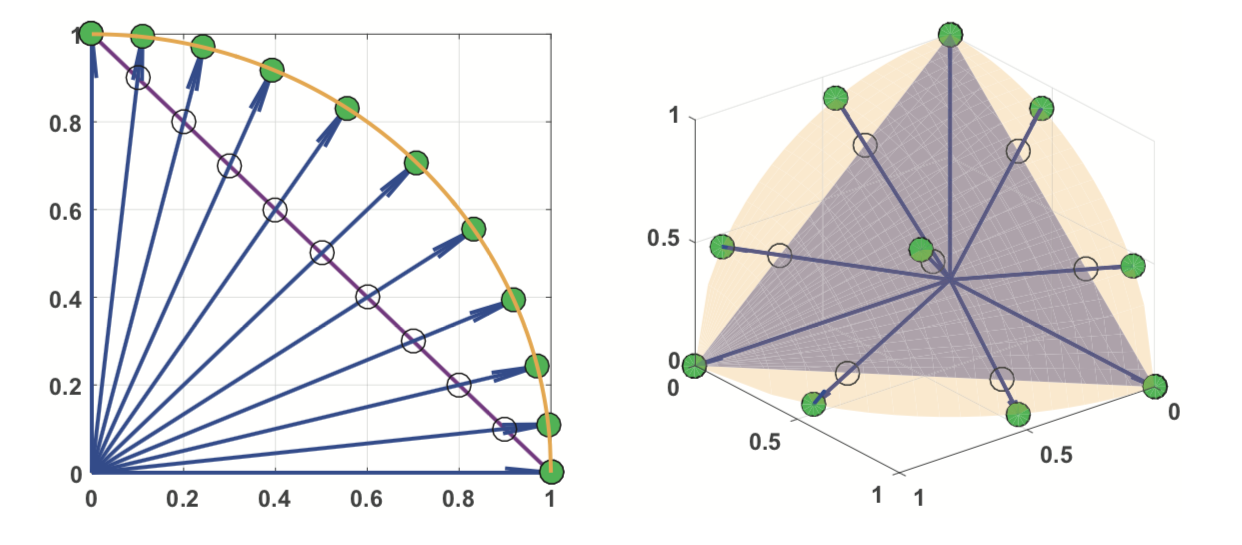
\includegraphics[width=\textwidth]{images/decomp2.png}
	\caption{Decomposition  -  2 and 3 objectives, \cite{chugh2017handling} }.
\end{figure*}

Why use decomposition?

It may be good at generating an even distribution of solutions in MOPs
It reduces the computation complexity when compared to other algorithms (NSGA-II) \cite{zhang2009performance}.
An optimal solution of a set of scalar optimization problems can be a Pareto optimal solution, under mild conditions
All solutions can be compared based on their objective function values
It is simple to find a solution to multi single-objective problems than for a multi-objective problem
Fitness assignment and diversity maintenance become easier to handle.

$f_{3}(x) = F * w_{3}$

In general, $f_{i}(x) = F * w_{i}$

\begin{figure*}[!t]
	\centering
	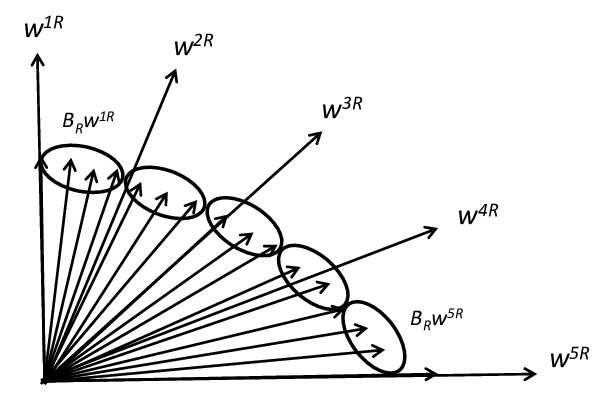
\includegraphics[width=\textwidth]{images/decomp.png}
	\caption{Decomposition and Aggregation Function - \cite{chugh2017handling}.}
\end{figure*}

Components of the MOEA/D

- Decomposition strategy: decomposes w/ weight vectors;
- Aggregation function:  weight vector => single-objective sub-problems;
- Neighbourhood assignment strategy: Relationship between sub-problems;
- Variation Stack: New candidates solutions;
- Update Strategy: Maintain/discard candidate solutions;
- Constraint handling method: Constraint violation;
- Termination Criteria: when to stop the search.

Variations Already Integrated

 On-line Resource Allocation - proposed in the context of MOEA/D by \cite{zhou2016all}.
 Bet-and-Run: A kind of restart strategy - in the context of single-objective problems (SOP) by \cite{friedrich2017generic}.

What is Online Resource Allocation 

- On-line Resource Allocation (ONRA) is an adaptation strategy that aim to adjust the behaviour of an algorithm in an on-line manner to suit the problem in question.


How it affects MOEA/D \cite{zhou2016all}.

- Some sub-problems can be more difficult to approximate that others. To better explore them, different computational resources are allocated to different sub-problems.

- The resources re-allocated is *the number of functions evaluations*.
- From an equal amount to every sub-problem to an amount related to the difficulty of the sub-problem.    


 Restart Strategy 


- Restart Strategy is a strategy used to avoid heavy-tailed running time distributions \cite{gomes2000heavy}.

-  If a execution of an algorithm does not conclude within a pre-determined limit or if the solution quality is unsatisfactory, we restart the algorithm @lissovoi2017theoretical.


Bet-and-Run framework 

- It is defined in @fischetti2014exploiting. as a number of short runs with randomized initial conditions, bet on the most promising run, and bring it to completion.

- To the best of our knowledge, only applied with EA in the context of SOP.

How it affects MOEA/D - \cite{lissovoi2017theoretical}.

- Initialisation can have a small beneficial effect even on very easy functions.

- Countermeasure when problems with promising and deceptive regions are encountered.

- Additional speed-up heuristic.